\heading{数据结构与算法B-21春-期末}
\textbf{一、选择题（30 分，每小题 2 分）}

\begin{question}
下列不影响算法时间复杂性的因素有（\quad）。
\begin{choiceoptions}[2]
  \item 问题的规模
  \item 输入值
  \item 计算结果
  \item 算法的策略
\end{choiceoptions}
\begin{solution}
选 C。算法时间复杂度由问题规模、输入数据和算法策略决定，与计算结果无关。
\end{solution}
\end{question}

\begin{question}
链表不具有的特点是（\quad）。
\begin{choiceoptions}[2]
  \item 可随机访问任意元素
  \item 插入和删除不需要移动元素
  \item 不必事先估计存储空间
  \item 所需空间与线性表长度成正比
\end{choiceoptions}
\begin{solution}
选 A。链表是顺序访问结构，不支持随机访问。
\end{solution}
\end{question}

\begin{question}
设有三个元素 $X,Y,Z$ 顺序进栈（进的过程中允许出栈），下列得不到的出栈排列是（\quad）。
\begin{choiceoptions}[2]
  \item $XYZ$
  \item $YZX$
  \item $ZXY$
  \item $ZYX$
\end{choiceoptions}
\begin{solution}
选 C。$ZXY$ 不可能：若 $Z$ 第一个出栈，则 $X,Y$ 已在栈中且 $Y$ 在栈顶，之后必须先出 $Y$ 再出 $X$，不能得到 $ZXY$。
\end{solution}
\end{question}

\begin{question}
判定一个队列 $Q$（申请数组空间为 $m$）为空的条件是（\quad）。
\begin{choiceoptions}[1]
  \item \texttt{Q.rear == Q.front}
  \item \texttt{Q.front != Q.rear}
  \item \texttt{Q.front == (Q.rear+1)\% m}
  \item \texttt{Q.front != (Q.rear+1)\%m}
\end{choiceoptions}
\begin{solution}
选 A。循环队列判空条件为 \texttt{rear == front}，判满条件为 \texttt{(rear+1)\%m == front}。
\end{solution}
\end{question}

\begin{question}
若定义二叉树中根结点的层数为 $0$，树的高度等于其结点的最大层数加一。则当某二叉树的前序遍历序列和后序遍历序列正好相反，则该二叉树一定是（\quad）。
\begin{choiceoptions}[2]
  \item 空或只有一个结点
  \item 高度等于其结点数
  \item 任一结点无左孩子
  \item 任一结点无右孩子
\end{choiceoptions}
\begin{solution}
选 B。先序和后序相反意味着每层只有一个结点，树退化为单链，高度等于结点数。
\end{solution}
\end{question}

\begin{question}
任意一棵二叉树中，所有叶结点在前序遍历序列、中序遍历序列和后序遍历序列中的相对次序（\quad）。
\begin{choiceoptions}[2]
  \item 发生改变
  \item 不发生改变
  \item 不能确定
  \item 以上都不对
\end{choiceoptions}
\begin{solution}
选 B。叶子结点在三种遍历中均保持从左到右的相对顺序。
\end{solution}
\end{question}

\begin{question}
假设线性表中每个元素有两个数据项 key1 和 key2，现对线性表按以下规则进行排序：先根据 key1 的值进行非递减排序；在 key1 值相同的情况下，再根据 key2 的值进行非递减排序。满足这种要求的排序方法是（\quad）。
\begin{choiceoptions}[1]
  \item 先按 key1 冒泡排序，再按 key2 直接选择排序
  \item 先按 key2 冒泡排序，再按 key1 直接选择排序
  \item 先按 key1 直接选择排序，再按 key2 冒泡排序
  \item 先按 key2 直接选择排序，再按 key1 冒泡排序
\end{choiceoptions}
\begin{solution}
选 D。两关键字排序通常应先按次要关键字 key2 排序，再按主要关键字 key1 进行稳定排序。冒泡排序稳定，能在第二趟按 key1 排序时保留 key1 相同记录之间的 key2 次序；直接选择排序通常不稳定，因此不能放在第二趟作为主关键字排序。
\end{solution}
\end{question}

\begin{question}
有 $n$ 个整数，找到其中最小整数需要比较次数至少是（\quad）次。
\begin{choiceoptions}[2]
  \item $n$
  \item $\log_2 n$
  \item $n^2-1$
  \item $n-1$
\end{choiceoptions}
\begin{solution}
选 D。找最小值至少需要 $n-1$ 次比较（每个元素至少参与一次比较，锦标赛形式）。
\end{solution}
\end{question}

\begin{question}
$n$ 个顶点的无向完全图的边数为（\quad）。
\begin{choiceoptions}[2]
  \item $n(n-1)$
  \item $n(n+1)$
  \item $n(n-1)/2$
  \item $n(n+1)/2$
\end{choiceoptions}
\begin{solution}
选 C。无向完全图每对顶点间有一条边，共 $C_n^2 = n(n-1)/2$ 条。
\end{solution}
\end{question}

\begin{question}
设无向图 $G=(V,E)$，$G'=(V',E')$，如果 $G'$ 是 $G$ 的生成树，则下面说法中错误的是（\quad）。
\begin{choiceoptions}[2]
  \item $G'$ 是 $G$ 的子图
  \item $G'$ 是 $G$ 的连通分量
  \item $G'$ 是 $G$ 的极小连通子图且 $V=V'$
  \item $G'$ 是 $G$ 的一个无环子图
\end{choiceoptions}
\begin{solution}
选 B。生成树是包含所有顶点的极小连通子图，但不一定是连通分量（连通分量是极大连通子图）。
\end{solution}
\end{question}

\begin{question}
有一个散列表，其散列函数为 $h(\mathrm{key})=\mathrm{key}\bmod 13$，使用再散列函数 $h_2(\mathrm{key})=\mathrm{key}\bmod 3$ 解决碰撞。当前散列表状态如下，其中空白表示该地址尚未存放关键码：
\[
\begin{array}{c|ccccccccccccc}
\text{地址} &0&1&2&3&4&5&6&7&8&9&10&11&12\\ \hline
\text{关键码} &&38&&&&&&&&&&&25
\end{array}
\]
从表中检索关键码 $38$ 需进行几次关键码比较（\quad）。
\begin{choiceoptions}[1]
  \item $1$
  \item $2$
  \item $3$
  \item $4$
\end{choiceoptions}
\begin{solution}
选 B。$h(38)=38\bmod13=12$，第一次比较地址 $12$ 中的 $25$，不匹配；步长为 $h_2(38)=2$，下一探查地址为 $(12+2)\bmod13=1$，第二次比较找到 $38$。
\end{solution}
\end{question}


\begin{question}
在一棵度为 $3$ 的树中，度为 $3$ 的结点个数为 $2$，度为 $2$ 的结点个数为 $1$，则度为 $0$ 的结点个数为（\quad）。
\begin{choiceoptions}[2]
  \item $4$
  \item $5$
  \item $6$
  \item $7$
\end{choiceoptions}
\begin{solution}
选 C。树中总边数 $=$ 总度数 $=3\times2+2\times1+n_1$，总结点数 $=2+1+n_1+n_0$，由边数 $=$ 结点数 $-1$ 得 $n_0=6$。
\end{solution}
\end{question}

\begin{question}
由同一组关键字集合构造的各棵二叉排序树（\quad）。
\begin{choiceoptions}[2]
  \item 其形态不一定相同，但平均查找长度相同
  \item 其形态不一定相同，平均查找长度也不一定相同
  \item 其形态均相同，但平均查找长度不一定相同
  \item 其形态均相同，平均查找长度也都相同
\end{choiceoptions}
\begin{solution}
选 B。BST 形态取决于插入顺序，不同形态影响查找效率。
\end{solution}
\end{question}

\begin{question}
允许表达式内多种括号混合嵌套，检查表达式中括号是否正确配对的算法，通常选用（\quad）。
\begin{choiceoptions}[2]
  \item 栈
  \item 线性表
  \item 队列
  \item 二叉排序树
\end{choiceoptions}
\begin{solution}
选 A。栈的后进先出特性适合括号匹配检查。
\end{solution}
\end{question}

\begin{question}
下列选项中最适合实现数据的频繁增删及高效查找的组织结构是（\quad）。
\begin{choiceoptions}[2]
  \item 有序表
  \item 堆排序
  \item 二叉排序树
  \item 快速排序
\end{choiceoptions}
\begin{solution}
选 C。BST 支持 $O(\log n)$ 的查找与 $O(\log n)$ 的插入/删除（平均情况）。
\end{solution}
\end{question}




\textbf{二、判断题（10 分，每小题 1 分；对 Y，错 N）}

\begin{question}
考虑一个长度为 $n$ 的顺序表中各个位置插入新元素的概率相同，则顺序表的插入算法平均时间复杂度为 $O(n)$。（\quad）
\begin{solution}
答案：Y。顺序表插入时，需要把插入位置及其后的元素整体后移。若插入到第 $i$ 个位置后面，则移动元素个数与 $i$ 有关；各位置等概率时，平均移动次数约为 $n/2$，因此平均时间复杂度为 $O(n)$。
\end{solution}
\end{question}

\begin{question}
希尔排序算法的每一趟都要调用一次或多次直接插入排序算法，所以其效率比直接插入排序算法差。（\quad）
\begin{solution}
答案：N。希尔排序虽然在每个增量分组内使用直接插入排序思想，但它先让相隔较远的元素交换，使序列逐步趋于有序；后续增量变小时，插入排序的代价会明显降低。因此不能因为“调用插入排序”就判断它一定更差。
\end{solution}
\end{question}

\begin{question}
直接插入排序、冒泡排序、Shell 排序都是在数据正序的情况下比数据在逆序的情况下要快。（\quad）
\begin{solution}
答案：Y。直接插入排序在正序时几乎不移动元素；带提前结束标志的冒泡排序在正序时一趟即可结束；Shell 排序在序列较有序时分组插入的移动量也更小。逆序通常导致更多比较和移动。
\end{solution}
\end{question}

\begin{question}
由于碰撞的发生，基于散列表的检索仍然需要进行关键码对比，并且关键码的比较次数仅取决于选择的散列函数与处理碰撞的方法两个因素。（\quad）
\begin{solution}
答案：N。散列表检索次数不仅与散列函数和冲突处理方法有关，还与装填因子、关键字分布、已有冲突链或探查序列长度有关。装填因子越高，平均冲突和比较次数往往越多。
\end{solution}
\end{question}

\begin{question}
若有一个叶子结点是二叉树中某个子树的前序遍历结果序列的最后一个结点，则它一定是该子树的中序遍历结果序列的最后一个结点。（\quad）
\begin{solution}
答案：N。反例：某子树根为 $A$，只有左孩子 $B$。其前序遍历为 $A,B$，最后一个结点 $B$ 是叶子；但中序遍历为 $B,A$，最后一个结点是根 $A$。所以该命题不成立。
\end{solution}
\end{question}

\begin{question}
若某非空二叉树的前序遍历序列和后序遍历序列正好相同，则该二叉树只有一个根结点。（\quad）
\begin{solution}
答案：Y。前序遍历第一个结点一定是根，后序遍历最后一个结点一定是根。若两序列完全相同，则第一个结点也必须等于最后一个结点；非空且结点互异时，只能说明序列长度为 $1$，即二叉树只有根结点。
\end{solution}
\end{question}

\begin{question}
有 $n$ 个结点的二叉排序树有多种；若按最坏情况下的查找比较次数衡量，树高最小的二叉排序树搜索效率最好。（\quad）
\begin{solution}
答案：Y。二叉排序树查找时，每向下一层就多比较一次，最坏比较次数与树高成正相关。树高越小，最坏情况下从根到叶的路径越短，因此按最坏情况衡量搜索效率更好。
\end{solution}
\end{question}

\begin{question}
强连通分量是有向图中的最小强连通子图。（\quad）
\begin{solution}
答案：N。强连通分量是有向图中的\textbf{极大}强连通子图，即再加入任何相邻顶点都会破坏强连通性；它不是“最小”强连通子图。单个顶点也可看作强连通子图，但通常不是强连通分量。
\end{solution}
\end{question}

\begin{question}
用邻接矩阵法存储一个图时，在不考虑压缩存储的情况下，所占用的存储空间大小只与图中结点个数有关，而与图的边数无关。（\quad）
\begin{solution}
答案：Y。邻接矩阵为每一对顶点预留一个表项，若图有 $n$ 个顶点，则矩阵大小为 $n\times n$。无论边多还是边少，都要存储这个矩阵，因此空间复杂度为 $O(n^2)$，与边数无关。
\end{solution}
\end{question}

\begin{question}
若定义一个有向图的根是指可以从这个结点到达图中任意其他结点，\par
则可知一个有向图中至少有一个根。（\quad）
\begin{solution}
答案：N。有向图不一定存在能到达所有其他顶点的结点。例如两个互不连通的强连通分量之间没有路径时，任何一个顶点都无法到达另一分量中的顶点，因此不存在这样的根。
\end{solution}
\end{question}

\textbf{三、填空题（20 分，每题 2 分）}

\begin{question}
线性表的顺序存储与链式存储是两种常见存储形式；当表元素有序排序进行二分检索时，应采用 \blank 存储形式。
\begin{solution}
答案：顺序存储。二分查找每一步都要直接访问中间位置元素，顺序表支持按下标随机访问，时间为 $O(1)$；链表只能从头顺序扫描到中间结点，无法高效二分。
\end{solution}
\end{question}

\begin{question}
设环形队列的容量为 $20$（单元编号 $0$ 到 $19$），经过一系列的入队和出队运算后，队头变量 front=18，队尾变量 rear=11，则环形队列中有 \blank 个元素。
\begin{solution}
答案：$13$。循环队列中元素个数通常计算为 $(rear-front+m)\bmod m$。代入 $m=20$ 得 $(11-18+20)\bmod20=13$。
\end{solution}
\end{question}

\begin{question}
一棵含有 $101$ 个结点的二叉树中有 $36$ 个叶子结点，度为 $2$ 的结点个数是 \blank，度为 $1$ 的结点个数是 \blank。
\begin{solution}
答案：$35$，$30$。二叉树中叶子数 $n_0$ 与度为 $2$ 的结点数 $n_2$ 满足 $n_0=n_2+1$，故 $n_2=36-1=35$。总结点数 $n=n_0+n_1+n_2$，所以 $n_1=101-36-35=30$。
\end{solution}
\end{question}

\begin{question}
已知二叉树的前序遍历结果为 $ADC$，这棵二叉树的树型有 \blank 种可能。
\begin{solution}
答案：$5$。只有前序序列且含 $3$ 个互异结点时，不能唯一确定二叉树形态。含 $3$ 个结点的二叉树形态数为 Catalan 数 $C_3=\dfrac{1}{4}\binom{6}{3}=5$。
\end{solution}
\end{question}

\begin{question}
已知二叉树的中序序列为 $DGBAECF$，后序序列为 $GDBEFCA$，该二叉树的先序序列是 \blank。
\begin{solution}
答案：\texttt{ABDGCEF}。后序最后一个结点 $A$ 为根；中序按 $A$ 分为左子树 $DGB$ 和右子树 $ECF$。左子树后序为 $GDB$，根为 $B$，其左子树为 $DG$；继续递归得到左子树先序 $B,D,G$。右子树后序为 $EFC$，根为 $C$，其左子树为 $E$、右子树为 $F$。合并得到先序 $A,B,D,G,C,E,F$。
\end{solution}
\end{question}

\begin{question}
对于具有 $57$ 个结点的完全二叉树，按层次自顶向下、同一层自左向右、从 $0$ 开始编号。编号为 $18$ 的结点的父结点编号为 \blank，编号为 $19$ 的结点的右子女结点编号为 \blank。
\begin{solution}
答案：$8$，$40$。从 $0$ 开始编号的完全二叉树中，结点 $i$ 的父结点编号为 $\lfloor(i-1)/2\rfloor$，右孩子编号为 $2i+2$。故 $18$ 的父结点为 $\lfloor17/2\rfloor=8$，$19$ 的右孩子为 $2\times19+2=40$；由于 $40\le 56$，该孩子存在。
\end{solution}
\end{question}

\begin{question}
有 $n$ 个数据对象的二路归并排序中，每趟归并的时间复杂度为 \blank。
\begin{solution}
答案：$O(n)$。二路归并排序的一趟归并会把当前各有序子序列两两合并，所有元素在这一趟中总共被扫描和移动常数次，因此每趟代价与元素总数成线性关系。
\end{solution}
\end{question}

\begin{question}
对一组记录进行降序排序，其关键码为 $(46,70,56,38,40,80,60,22)$，采用初始步长为 $4$ 的希尔排序，第一趟扫描的结果是 \blank，而采用归并排序第一轮归并的结果是 \blank。
\begin{solution}
答案：$(46,80,60,38,40,70,56,22)$；$(70,46,56,38,80,40,60,22)$。希尔排序第一趟按步长 $4$ 分组，比较 $(46,40)$、$(70,80)$、$(56,60)$、$(38,22)$ 并按降序整理，得到第一组结果。归并排序第一轮把相邻单元素两两按降序归并，所以 $(46,70)$ 变为 $(70,46)$，$(56,38)$ 不变，$(40,80)$ 变为 $(80,40)$，$(60,22)$ 不变。
\end{solution}
\end{question}

\begin{question}
如果只想得到 $1000$ 个元素的序列中最小的前 $5$ 个元素，在冒泡排序、快速排序、堆排序和归并排序中，哪种算法最快？\blank
\begin{solution}
答案：堆排序。只需要前 $5$ 个最小元素时，不必完全排序。可建立小根堆后连续取出 $5$ 次堆顶，代价约为 $O(n+5\log n)$，比完整归并排序、快速排序或冒泡排序更适合该需求。
\end{solution}
\end{question}

\begin{question}
如果一个图结点多而边少（稀疏图），适宜采用 \blank 方式进行存储。
\begin{solution}
答案：邻接表。邻接矩阵固定占用 $O(n^2)$ 空间，而邻接表只保存顶点表和实际存在的边，空间为 $O(n+e)$。稀疏图中 $e$ 远小于 $n^2$，因此邻接表更节省空间。
\end{solution}
\end{question}

\textbf{四、简答题（24 分，每小题 6 分）}

\begin{question}[森林周游]（6 分）

树周游算法可以很好地应用到森林的周游上。查看下列森林结构，请给出其深度优先周游序列和广度优先周游序列。

\begin{center}
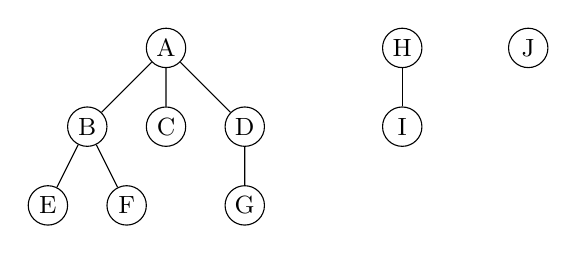
\begin{tikzpicture}[level distance=9mm,sibling distance=14mm,every node/.style={draw,circle,font=\small,minimum size=5mm,inner sep=0pt}]
\node (A) at (0,0) {A};
\node (B) at (-1,-1) {B}; \node (C) at (0,-1) {C}; \node (D) at (1,-1) {D};
\node (E) at (-1.5,-2) {E}; \node (F) at (-0.5,-2) {F}; \node (G) at (1,-2) {G};
\draw (A)--(B) (A)--(C) (A)--(D) (B)--(E) (B)--(F) (D)--(G);
\node (H) at (3,0) {H}; \node (I) at (3,-1) {I}; \draw (H)--(I);
\node (J) at (4.6,0) {J};
\end{tikzpicture}
\end{center}

\begin{solution}
深度优先周游按先根次序依次访问各树：第一棵树为 $A,B,E,F,C,D,G$，第二棵树为 $H,I$，第三棵树为 $J$，因此序列为
\[A,B,E,F,C,D,G,H,I,J.\]
广度优先周游先访问各棵树的根，再逐层从左到右访问，序列为
\[A,H,J,B,C,D,I,E,F,G.\]
\end{solution}
\end{question}

\begin{question}[Huffman树]（6 分）

设给定五个字符，其相应的权值分别为 $\{4,8,6,9,18\}$，试画出相应的哈夫曼树，并计算它的带权外部路径长度 WPL。

\begin{solution}
Huffman 树构建：每次合并权值最小的两个结点。
\begin{itemize}
  \item 合并 $4,6$ 得 $10$
  \item 合并 $8,9$ 得 $17$
  \item 合并 $10,17$ 得 $27$
  \item 合并 $18,27$ 得 $45$
\end{itemize}
WPL 等于各次合并权值之和：$10+17+27+45=99$。等价地，$4,6,8,9$ 的深度为 $3$，$18$ 的深度为 $1$，故 $WPL=4\times3+6\times3+8\times3+9\times3+18\times1=99$。
\end{solution}
\end{question}

\begin{question}[堆操作]（6 分）

下图是一棵完全二叉树：
\begin{center}
\begin{tikzpicture}[x=1cm,y=1cm,every node/.style={font=\normalsize,inner sep=1pt}]
\node (n1) at (0,0) {31};
\node (n2) at (-2,-1) {8};
\node (n3) at (2,-1) {53};
\node (n4) at (-3,-2) {10};
\node (n5) at (-1,-2) {20};
\node (n6) at (1,-2) {7};
\node (n7) at (3,-2) {15};
\node (n8) at (-3.5,-3) {3};
\node (n9) at (-2.5,-3) {20};
\node (n10) at (-1,-3) {1};
\foreach \a/\b in {n1/n2,n1/n3,n2/n4,n2/n5,n3/n6,n3/n7,n4/n8,n4/n9,n5/n10}
  \draw (\a)--(\b);
\end{tikzpicture}
\end{center}

\begin{enumerate}[label=\arabic*)]
  \item 请根据初始建堆算法对该完全二叉树建堆，请画出构建的小根堆；（2 分）
  \item 基于（1）中得到的堆，删除其中的最小元素，请用图给出堆的调整过程；（2 分）
  \item 基于（1）中得到的堆，向其中插入元素 $2$，请给出堆的调整过程。（2 分）
\end{enumerate}

\begin{solution}
\begin{enumerate}[label=\arabic*)]
  \item 原树按层次序列为 $(31,8,53,10,20,7,15,3,20,1)$。自最后一个非叶结点向前下滤，可得小根堆层次序列
  \[ (1,3,7,10,8,53,15,31,20,20). \]
  \begin{center}
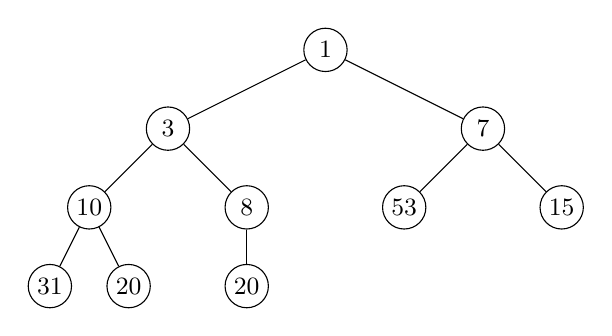
\begin{tikzpicture}[x=1cm,y=1cm,every node/.style={draw,circle,font=\small,minimum size=5.5mm,inner sep=0pt}]
\node (h1) at (0,0) {1};
\node (h2) at (-2,-1) {3};
\node (h3) at (2,-1) {7};
\node (h4) at (-3,-2) {10};
\node (h5) at (-1,-2) {8};
\node (h6) at (1,-2) {53};
\node (h7) at (3,-2) {15};
\node (h8) at (-3.5,-3) {31};
\node (h9) at (-2.5,-3) {20};
\node (h10) at (-1,-3) {20};
\foreach \a/\b in {h1/h2,h1/h3,h2/h4,h2/h5,h3/h6,h3/h7,h4/h8,h4/h9,h5/h10}
  \draw (\a)--(\b);
\end{tikzpicture}
\end{center}
  \item 删除最小元素 $1$ 后，以末尾元素 $20$ 补到根并下滤：
  \[ (20,3,7,10,8,53,15,31,20)\to(3,8,7,10,20,53,15,31,20). \]
  \item 插入 $2$ 后先放在末尾，再依次与父结点 $8,3$ 交换，结果为
  \[ (1,2,7,10,3,53,15,31,20,20,8). \]
\end{enumerate}
\end{solution}
\end{question}

\begin{question}[Prim算法求最小生成树]（6 分）

已知图 $G$ 的顶点集合 $V=\{V_0,V_1,V_2,V_3,V_4\}$，邻接矩阵如下（$\infty$ 表示无边）：
\[
\begin{pmatrix}
0 & 7 & \infty & 4 & 2\\
7 & 0 & 9 & 1 & 5\\
\infty & 9 & 0 & 3 & \infty\\
4 & 1 & 3 & 0 & 10\\
2 & 5 & \infty & 10 & 0
\end{pmatrix}
\]

\begin{enumerate}[label=\arabic*)]
  \item 根据 Prim 算法，求图 $G$ 从顶点 $V_0$ 出发的最小生成树；（2 分）
  \item 给出每一步执行后的 mst 数组。（4 分）
\end{enumerate}

\begin{solution}
从 $V_0$ 出发，逐步选择跨越当前顶点集的最小边。执行状态如下，其中 $U$ 表示已加入生成树的顶点集，$lowcost$ 为到 $U$ 的最小边权。
\begin{center}
\small
\begin{tabular}{c c c c}
\toprule
步骤 & 新加入顶点 & $U$ & 当前最小边 \\ 
\midrule
初始 & $V_0$ & $\{V_0\}$ & - \\ 
1 & $V_4$ & $\{V_0,V_4\}$ & $(V_0,V_4),2$ \\ 
2 & $V_3$ & $\{V_0,V_4,V_3\}$ & $(V_0,V_3),4$ \\ 
3 & $V_1$ & $\{V_0,V_4,V_3,V_1\}$ & $(V_3,V_1),1$ \\ 
4 & $V_2$ & $\{V_0,V_4,V_3,V_1,V_2\}$ & $(V_3,V_2),3$ \\ 
\bottomrule
\end{tabular}
\end{center}
因此最小生成树为 $\{(V_0,V_4),(V_0,V_3),(V_3,V_1),(V_3,V_2)\}$，总权值为 $10$。
\end{solution}
\end{question}

\textbf{五、算法题（16 分，每小题 8 分）}


\begin{question}[根据前序求后序]
下列 Python 函数的功能是：根据一个满二叉树的前序遍历序列，求其后序遍历序列。参数 \texttt{s} 为当前子树在前序序列中的起点，\texttt{length} 为当前子树结点数。请补全空白（假设序列长度不超过 $32$）。

\begin{pycode}
def preorder_to_postorder(seq, s, length):
    if length == 1:
        return __________                      # (1)

    sub_len = __________                       # (2)
    s1 = s + 1
    s2 = __________                            # (3)
    left = preorder_to_postorder(seq, s1, sub_len)
    right = __________                         # (4)
    return __________                          # (5)
\end{pycode}

\begin{solution}
填空答案：
\begin{enumerate}
  \item \texttt{seq[s]}
  \item \texttt{(length - 1) // 2}
  \item \texttt{s + sub\_len + 1}
  \item \texttt{preorder\_to\_postorder(seq, s2, sub\_len)}
  \item \texttt{left + right + seq[s]}
\end{enumerate}
满二叉树左右子树结点数相同，均为 $(\texttt{length}-1)/2$。前序序列的第一个元素是根，之后依次是左子树和右子树；后序遍历顺序为“左子树、右子树、根”，因此返回左、右子树后序结果再拼接根结点。
\end{solution}
\end{question}



\begin{question}[深度优先周游]
阅读下列 Python 程序，完成图的深度优先周游算法。图采用邻接表表示：\par
\texttt{graph["vertices"]} 存放顶点标记，\texttt{graph["adj"][i]} 存放顶点 $i$ 的所有邻接点编号。

\begin{pycode}
def dfs_in_list(graph, visited, i):
    print(f"node: {graph['vertices'][i]}")
    visited[i] = True
    for j in __________:                       # (1)
        if __________:                         # (2)
            __________                         # (3)


def traverse_dfs(graph):
    n = len(graph["vertices"])
    visited = [False] * n
    for i in range(n):
        if __________:                         # (4)
            dfs_in_list(graph, visited, i)
\end{pycode}

\begin{solution}
填空答案：
\begin{enumerate}
  \item \texttt{graph["adj"][i]}
  \item \texttt{not visited[j]}
  \item \texttt{dfs\_in\_list(graph, visited, j)}
  \item \texttt{not visited[i]}
\end{enumerate}
DFS 的核心是：访问当前顶点后，依次扫描当前顶点邻接表中的顶点；对尚未访问的邻接点递归。外层循环保证即使图不连通，也能从每个未访问顶点启动一次 DFS，从而完成全图周游。
\end{solution}
\end{question}



